%\documentclass[a4, semhelv, semrot,portrait]{seminar}
\documentclass[a4, semhelv, semrot, landscape]{seminar} 
\usepackage[dvips]{graphicx}
\usepackage{fancybox}
\usepackage{a4wide} 
\usepackage{amsmath} 
\usepackage{amsxtra} 

%\def\printlandscape{\special{landscape}}
%\landscapeonly
%\slideframe{Oval}
%\renewcommand{\printlandscape}{\special{landscape}}
%\include{sem-a4.sty}

\newcommand{\heading}[1]{\begin{center}%
                        {\Large {\bf \sffamily{ #1 }}}\\[2mm]%
                        \hrule\vspace{2mm}
                        \end{center}}
\begin{document}

\begin{slide}
    \begin{center}
    \rule{\textwidth}{1mm}
    {\bf \Large{Atomic Form Factors\\ and X Ray -- Atom Scattering}} \\[1mm]
    \rule{\textwidth}{1mm} %\vspace{5cm}
    \\[2cm]
    \large{
    Michael Papasimeon\\
    1998 Proposed Honours Project\\
    Supervisor : Dr. Chris Chantler}
    \end{center}
\end{slide}

\begin{slide}
    \heading{Photon-Atom Scattering}
    \begin{itemize}
        \item Interested at how X ray scatter off a single atom
        \item The types of scattering processes include
        \begin{itemize}
            \item Elastic (Rayleigh) Scattering
            \item Inelastic (Compton) Scattering
            \item Photo Effect
            \item Pair Production
            \item Nuclear Thomson Scattering
        \end{itemize}
%        \item In the X ray region ( $<$ 100 keV), Rayleigh, Compton and
%              Photo Effect are the dominant processes.
    \end{itemize}
    \begin{center}
        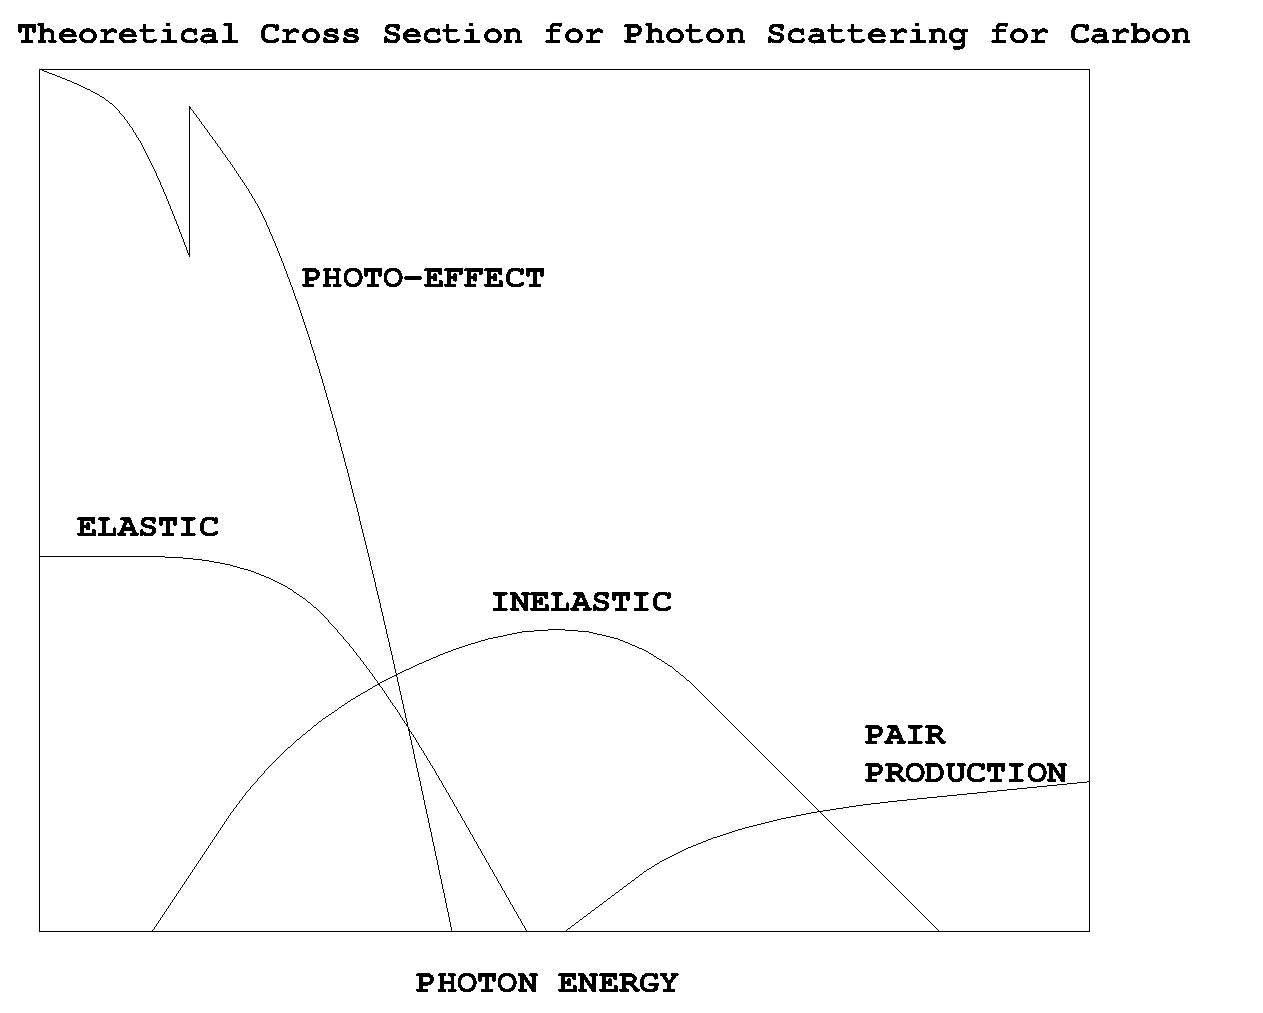
\includegraphics[width=6cm]{cross_section.eps}
    \end{center}
\end{slide}

\begin{slide}
    \heading{Scattering Amplitudes}
    \begin{itemize}
    \item Schr\"odinger Equation for a scattering process
        \[ [ H_0 + H'] \psi = E \psi\]
    \item Scattering Wave Function as $r \rightarrow \infty$ can be considered
          as an incident and scattered wave.
    \[ \psi(r) = \psi_i(r) + \psi_s(r)\]
    \[ \psi(r) = A \left[ e^{ik \cdot r}  + 
                    f(k,\theta, \phi) \frac{e^{ikr}}{r} \right] \]
    \item $f(k,\theta, \phi)$ is the scattering amplitude
    \item Differential Cross Section
        \[ \frac{d \sigma}{d \Omega} = | f(k, \theta, \phi) |^2 \]
    \end{itemize}
\end{slide}

\begin{slide}
    \heading{Relevance of Atomic Form Factors}
    \begin{itemize}
        \item The scattering amplitude depends on the atomic
              form factor
        \item Scattering amplitude -- form factor relationship
              depends on how atom-radiation interaction is modeled
        \item Atomic Form Factors are used to determine diffraction,
              scattering and attenuation processes of X ray interactions
              with matter.
    \end{itemize}
\end{slide}

\begin{slide}
    \heading{Definition of Atomic Form Factors}
    \begin{itemize}
        \item Total Atomic Form Factor
            \[ f = f_0 + f' + if'' \]
        \item Away from absorption edges (for a spherically symmetric atom)
            \[ f_0(q) = \int e^{i q r} \rho(r) dr
                      = 4 \pi \int_{0}^{\infty} \rho(r) \frac{\sin qr}{qr} r^2 dr
            \]
        \item $q = k_f - k_i = 2|k| \sin \left (\frac{\theta}{2} \right)$ 
                is the change in the photon's momentum and $\theta$ is the
                scattering angle.
        \item $\rho(r) = \psi^{*}(r) \psi(r)$ is the electron density.
        \item The real and imaginary components $f'$ and $f''$ describe 
              the situation when
              the photon energy is close to one of the atom's energy levels
              -- an absorption edge.
    \end{itemize}
\end{slide}

\begin{slide}
    \heading{Examples of Atomic Form Factors}
    \begin{center}
        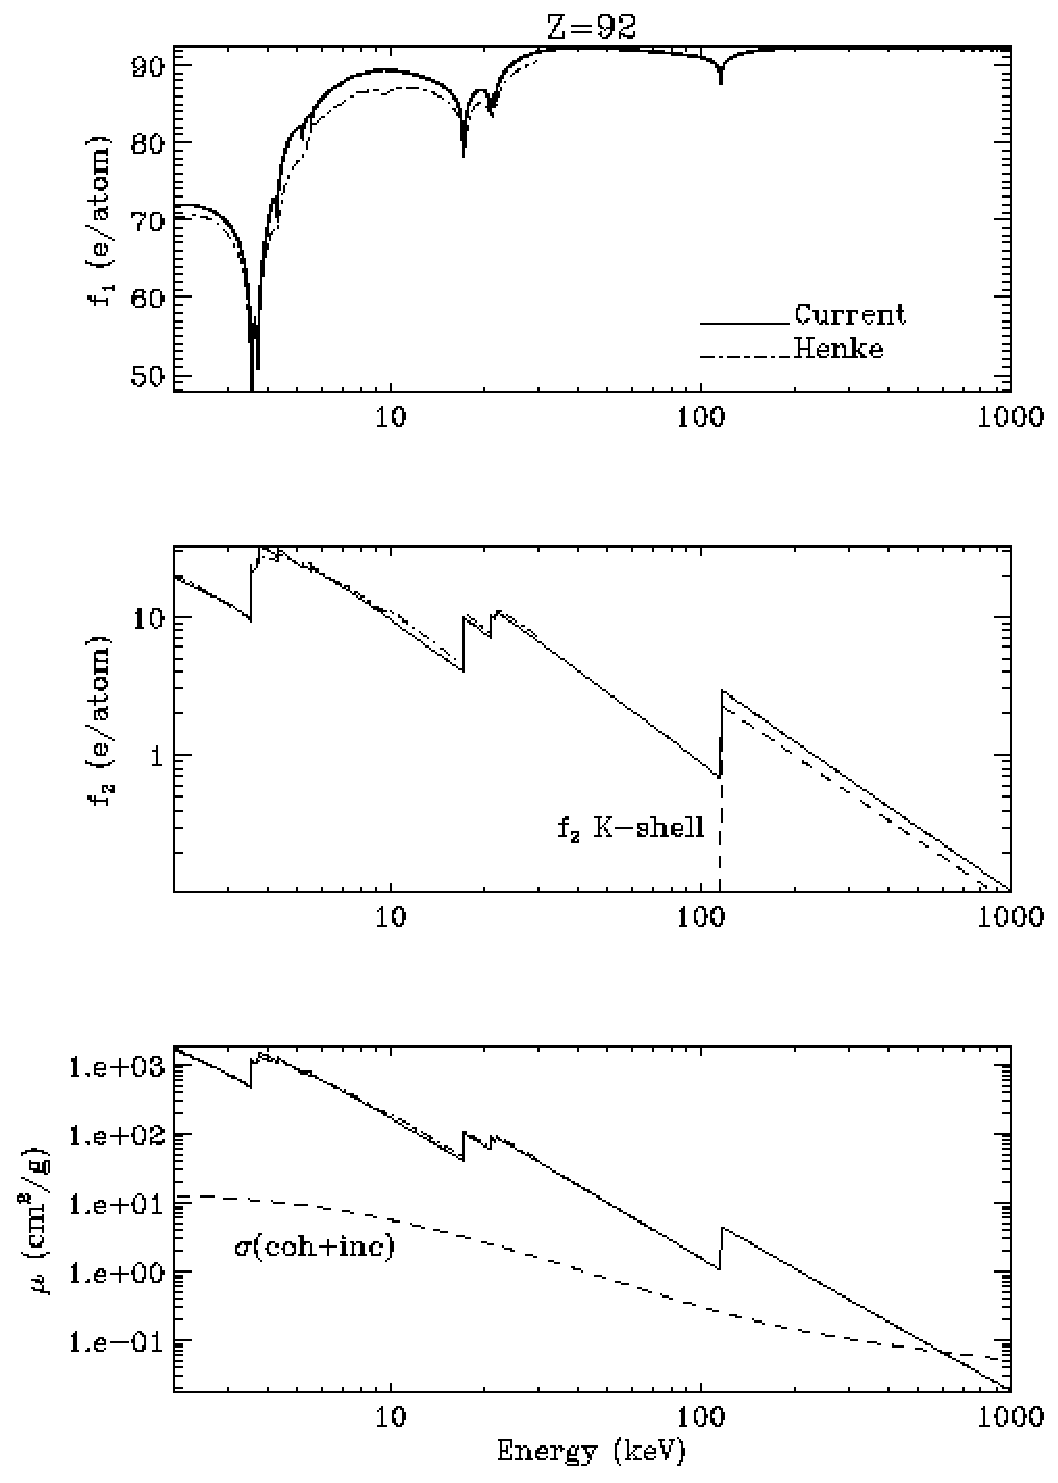
\includegraphics[width=4cm]{form_factor.eps}
    \end{center}
\end{slide}

\begin{slide}
    \heading{Scattering from Multiple Atoms}
    Experiments deal with many atoms, and there are a number
    of effects which cannot be explained by treating the atom
    as an isolated system.
    \begin{itemize}
        \item Extended X-ray Anomalous Fine Structure (EXAFS)
        \item X-ray Anomalous Near Edge Structure (XANES)
    \end{itemize}
    \begin{center}
        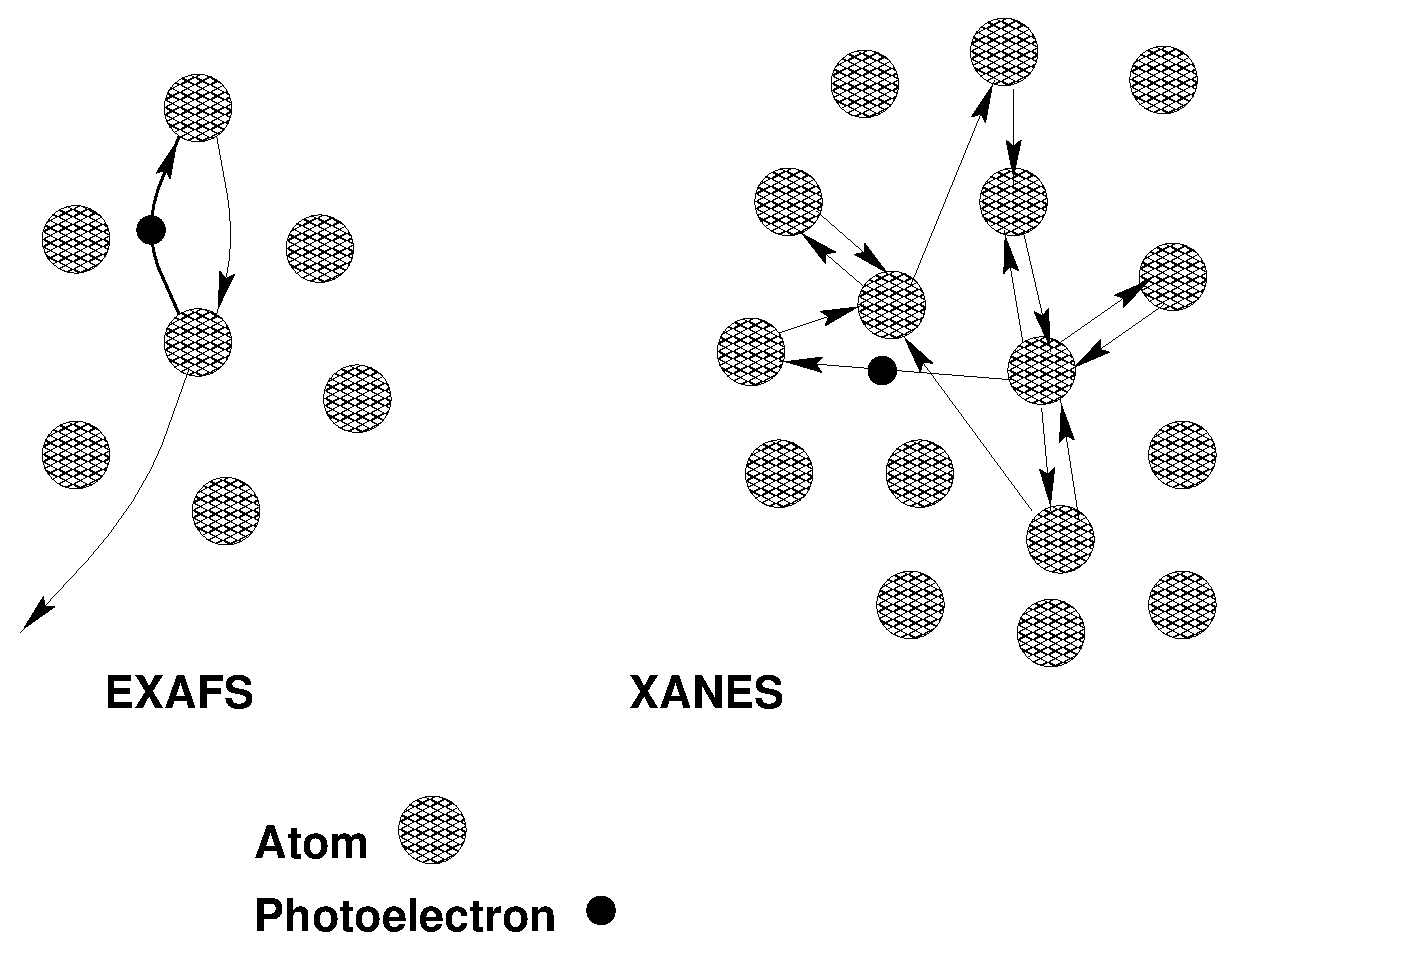
\includegraphics[width=5cm]{exafs.eps}
    \end{center}
\end{slide}

\begin{slide}
    \heading{Existing Theoretical And Experimental Results}
    \begin{itemize}
        \item {\bf THEORY}
            \begin{itemize}
                \item Partially-Relativistic Quantum Mechanics
                    \begin{itemize}
                        \item Hubbel, Scofield
                    \end{itemize}
                \item Relativistic Quantum Mechanics
                    \begin{itemize}
                        \item Dirac-Hartree-Fock, {\it S}-Matrix,   
                              Relativistic Multipole etc.
                        \item Cromer and Liberman, Kissel and Pratt,
                              Creagh, Chantler
                    \end{itemize}
            \end{itemize}
        \item {\bf EXPERIMENT} -- Errors  of 10\% --20\% for best data
            \begin{itemize}
                \item Experimental Synthesis
                    \begin{itemize}
                        \item Henke, Gullikson
                    \end{itemize}
                \item Experimental Compilation
                    \begin{itemize}
                        \item Hubbel
                    \end{itemize}
            \end{itemize}
    \end{itemize}
\end{slide}

\begin{slide}
    \heading{Main Project Aims}
    \begin{itemize}
        \item Develop the theory for atomic form factors for low Z atoms.
        \item Determine atomic form factors for low Z atoms and compare with
              existing theories and experimental results.
        \item Investigate and develop the theory of anomalous X ray resonance
              scattering (EXAFS, XANES, DAFS) -- effects of local interactions
              on the atomic form factor.
    \end{itemize}
\end{slide}

\begin{slide}
    \heading{Proposed Approach}
    \begin{itemize}
        \item Atom -- Relativistic Quantum Mechanics (Dirac) 
        \item X Ray -- Classical Radiation Field using 
              electric dipole and/or electric quadrupole approximation 
        \item Investigate the effect of local interactions on the atomic form factor
        \item Use a Dirac-Hartree-Fock computational approach to determine
              for multi-electron atoms the
              \begin{itemize}
                \item Energy eigenvalues of the atom 
                \item Corresponding wave functions
              \end{itemize}
        \item Use these wave functions to determine the atomic form factors
              for the different atoms over a range of X ray energies.
              \begin{itemize}
                \item Angular dependent component of the atomic form factor $f_0$
                \item Energy dependent components of the atomic form factor
                      $f'$ and $f''$
              \end{itemize}
    \end{itemize}
\end{slide}


\end{document}

